\documentclass[border=10pt]{standalone}
\usepackage{tikz}
\usetikzlibrary{shapes.geometric, arrows.meta, calc}
\usepackage{pifont}
\usepackage{amsmath}
\usepackage{fontawesome5}

\begin{document}
\begin{tikzpicture}[
    >=stealth,
    font=\sffamily\footnotesize,
    lm_outer/.style={rectangle, draw=blue!60!black, fill=blue!15, thick, rounded corners=4mm, minimum width=4cm, minimum height=5.5cm, align=center},
    lm_inner/.style={rectangle, fill=cyan!5, rounded corners=2mm, minimum width=3.4cm, minimum height=4cm},
    input_box/.style={rectangle, draw=orange!50, fill=orange!20, rounded corners=1mm, text width=5cm, inner sep=4pt, align=left},
    ans_box/.style={rectangle, draw=orange!50, fill=orange!20, font=\bfseries, inner sep=4pt},
    q_h_box/.style={rectangle, draw=yellow!80!orange, fill=yellow!30, rounded corners=1.5mm, minimum width=3cm, minimum height=4mm},
    trap_A_old/.style={trapezium, draw=teal!80!black, fill=green!10, trapezium angle=65, thick, minimum width=1.5cm, minimum height=0.7cm, align=center, shape border rotate=180},
    trap_B_old/.style={trapezium, draw=teal!80!black, fill=green!10, trapezium angle=65, thick, minimum width=1.5cm, minimum height=0.7cm, align=center},
    trap_A_new/.style={trapezium, draw=blue!80!black, fill=blue!10, trapezium angle=65, thick, minimum width=1.5cm, minimum height=0.7cm, align=center, shape border rotate=180},
    trap_B_new/.style={trapezium, draw=blue!80!black, fill=blue!10, trapezium angle=65, thick, minimum width=1.5cm, minimum height=0.7cm, align=center},
    var_w/.style={rectangle, draw=blue!80!black, fill=cyan!10, minimum size=6mm, inner sep=2pt, align=center},
    var_a_old/.style={rectangle, draw=teal!80!black, fill=green!15, minimum size=5mm, inner sep=2pt},
    var_a_new/.style={rectangle, draw=blue!80!black, fill=blue!15, minimum size=5mm, inner sep=2pt},
    gate_old/.style={rectangle, draw=black, thick, fill=gray!20, rounded corners=2mm, minimum width=1.8cm, minimum height=1.2cm, align=center},
    gate_new/.style={rectangle, draw=red!80!black, thick, fill=gray!20, rounded corners=2mm, minimum width=1.8cm, minimum height=1.2cm, align=center},
    const_box/.style={rectangle, draw=blue!80!black, fill=blue!10, text width=1.8cm, align=center, minimum height=0.9cm},
    step_box/.style={rectangle, draw=blue!40, fill=blue!10, text width=2.8cm, align=left, inner sep=3pt},
    plus_op/.style={circle, draw=black, thick, fill=white, inner sep=0pt, minimum size=4.5mm},
    times_op/.style={circle, draw=black, thick, fill=white, inner sep=0pt, minimum size=4.5mm}
]

% =======================================================
% PHẦN (a) - EXPANDABLE LORA ARCHITECTURE
% =======================================================

% 1. LM Box & Inputs
\node[input_box] (input_a) at (0, 0) {Someone who had a very bad flight might be given a trip in this to make up for it?\\ \textbf{Option:} (A)first class (B)propitious (C)reputable (D)one (E)sufficient};
\node[font=\large] at (-3, 0) {$\boldsymbol{x}$};

\node[lm_outer] (lm) at (0, 4.5) {};
\node[font=\bfseries] at (0, 6.8) {Language Models};
\node[lm_inner] (lm_in) at (0, 4.2) {};

\node[ans_box] (ans) at (0, 8.2) {Answer: A};
\draw[->, thick, line width=1.2pt] (0, 7.25) -- (ans.south);

\node[q_h_box] (h) at (0, 2.7) {};
\node at (-1.8, 2.7) {$\boldsymbol{h}$};
\node[q_h_box] (q) at (0, 5.7) {};
\node at (-1.8, 5.7) {$\boldsymbol{q}$};

\node[plus_op] (lm_plus) at (0, 4.2) {$\boldsymbol{+}$};
\node[rectangle, draw=black, fill=white, align=center, font=\scriptsize, minimum width=1.3cm] (W) at (-1.1, 4.2) {Pre-trained\\Weights\\$\boldsymbol{W}$\\\textcolor{cyan}{\ding{101}}};
\node[var_w] (wt_small) at (1.2, 4.2) {$w_t$};

\draw[->, thick, line width=1.2pt] (input_a.north) -- (h.south);
\draw[->, thick, line width=1.2pt] (h.north) -- (lm_plus.south);
\draw[->, thick, line width=1.2pt] (lm_plus.north) -- (q.south);

% 2. Big Expandable Box
\draw[black, thick, rounded corners=4mm] (3.5, -0.5) rectangle (16.5, 9);

\draw[dashed, thick] (1.5, 4.5) -- (3.5, 9);
\draw[dashed, thick] (1.5, 3.9) -- (3.5, -0.5);

% Legend
\node[plus_op, minimum size=4mm] at (6.5, 8.5) {$\boldsymbol{+}$}; 
\node at (7.5, 8.5) {Addition};
\node[times_op, minimum size=4mm] at (9.2, 8.5) {$\boldsymbol{\times}$}; 
\node at (10.4, 8.5) {Multiplication};
\node[text=cyan, font=\large] at (12, 8.5) {\ding{101}}; 
\node at (12.8, 8.5) {: Frozen};

% Đầu ra của Expandable Box
\node[var_w, minimum size=7mm] (wt_big) at (9.5, 7.5) {$w_t$};
\node[plus_op] (big_plus) at (9.5, 6) {$\boldsymbol{+}$};
\draw[->, thick, line width=1.5pt] (big_plus.north) -- (wt_big.south);

% Trục Bus ngang
\draw[thick, line width=1.5pt] (5.5, 4.8) -- (13.5, 4.8);
\draw[thick, line width=1.5pt] (9.5, 4.8) -- (big_plus.south);

% Background Old/New
\fill[green!15, rounded corners=2mm] (4, 0) rectangle (9.2, 4.5);
\node[font=\bfseries] at (6.6, -0.2) {Old Branches};

\fill[blue!15, rounded corners=2mm] (10.5, 0) rectangle (13.5, 4.5);
\node[font=\bfseries] at (12, -0.2) {New Branch};

% Nhánh 1 (X = 5.5)
\node[var_a_old] (a1) at (4.5, 4) {$a_1$};
\node[times_op] (t1_top) at (5.5, 4) {$\boldsymbol{\times}$};
\node[trap_A_old] (A1) at (5.5, 2.7) {$\boldsymbol{A_1}$\\ \tiny\textcolor{cyan}{\ding{101}}};
\node[times_op] (t1_bot) at (5.5, 1.5) {$\boldsymbol{\times}$};
\node[trap_B_old] (B1) at (5.5, 0.5) {$\boldsymbol{B_1}$\\ \tiny\textcolor{cyan}{\ding{101}}};

\draw[->, thick, line width=1.5pt] (B1.north) -- (t1_bot.south);
\draw[->, thick, line width=1.5pt] (t1_bot.north) -- (A1.south);
\draw[->, thick, line width=1.5pt] (A1.north) -- (t1_top.south);
\draw[->, thick, line width=1.5pt] (t1_top.north) -- (5.5, 4.8);
\draw[->, thick, line width=1.2pt] (a1.east) -- (t1_top.west);

% Dấu chấm lửng
\node[font=\large] at (7.2, 2.7) {$\boldsymbol{\dots}$};
\node[font=\large] at (7.2, 0.5) {$\boldsymbol{\dots}$};

% Nhánh t-1 (X = 8.4)
\node[var_a_old] (atm1) at (7.4, 4) {$a_{t-1}$};
\node[times_op] (ttm1_top) at (8.4, 4) {$\boldsymbol{\times}$};
\node[trap_A_old] (Atm1) at (8.4, 2.7) {$\boldsymbol{A_{t-1}}$\\ \tiny\textcolor{cyan}{\ding{101}}};
\node[times_op] (ttm1_bot) at (8.4, 1.5) {$\boldsymbol{\times}$};
\node[trap_B_old] (Btm1) at (8.4, 0.5) {$\boldsymbol{B_{t-1}}$\\ \tiny\textcolor{cyan}{\ding{101}}};

\draw[->, thick, line width=1.5pt] (Btm1.north) -- (ttm1_bot.south);
\draw[->, thick, line width=1.5pt] (ttm1_bot.north) -- (Atm1.south);
\draw[->, thick, line width=1.5pt] (Atm1.north) -- (ttm1_top.south);
\draw[->, thick, line width=1.5pt] (ttm1_top.north) -- (8.4, 4.8);
\draw[->, thick, line width=1.2pt] (atm1.east) -- (ttm1_top.west);

% Nhánh t (X = 12.5)
\node[var_a_new] (at) at (11.5, 4) {$a_t$};
\node[times_op] (tt_top) at (12.5, 4) {$\boldsymbol{\times}$};
\node[trap_A_new] (At) at (12.5, 2.7) {$\boldsymbol{A_t}$};
\node[times_op] (tt_bot) at (12.5, 1.5) {$\boldsymbol{\times}$};
\node[trap_B_new] (Bt) at (12.5, 0.5) {$\boldsymbol{B_t}$\\ \tiny\textcolor{red}{\faFire}};

\draw[->, thick, line width=1.5pt] (Bt.north) -- (tt_bot.south);
\draw[->, thick, line width=1.5pt] (tt_bot.north) -- (At.south);
\draw[->, thick, line width=1.5pt] (At.north) -- (tt_top.south);
\draw[->, thick, line width=1.5pt] (tt_top.north) -- (12.5, 4.8);
\draw[->, thick, line width=1.2pt] (at.east) -- (tt_top.west);

% Hộp chú thích Step
\node[step_box] (step2) at (15, 7.2) {\textbf{2.} Integrating new and\\old LoRA branches};
\draw[->, thick] (step2.west) -- (wt_big.east);

\node[step_box] (step1) at (15, 4.6) {\textbf{1.} Expanding a new\\LoRA branch};
% \draw[->, thick] (step1.west) -- (tt_top.east);

\node[step_box] (step3) at (15, 2) {\textbf{3.} Updating new\\branch to learn new\\task};
% \draw[->, thick] (step3.west) -- (tt_bot.east);

\node[font=\large\bfseries] at (8, -1.5) {(a) Expandable LoRA Architecture in GainLoRA};

% =======================================================
% PHẦN (b) - GATING MODULES
% =======================================================

\begin{scope}[shift={(21.5, 0)}]

    % Input
    \node[input_box] (input_b) at (4.5, 0) {Someone who had a very bad flight might be given a trip in this to make up for it?\\ \textbf{Option:} (A)first class (B)propitious (C)reputable (D)one (E)sufficient};
    \node[font=\large] at (1.5, 0) {$\boldsymbol{x}$};

    % Nền Gating
    \fill[green!15, rounded corners=2mm] (0.2, 1.8) rectangle (5.8, 3.5);
    \fill[blue!15, rounded corners=2mm] (7.5, 1.8) rectangle (10.5, 3.5);

    % Khối Gating
    \node[gate_old] (g1) at (1.5, 2.6) {$\boldsymbol{g_1(\cdot)}$\\ \tiny\textcolor{cyan}{\ding{101}}};
    \node[gate_old] (gtm1) at (4.5, 2.6) {$\boldsymbol{g_{t-1}(\cdot)}$\\ \tiny\textcolor{cyan}{\ding{101}}};
    \node[gate_new] (gt) at (9, 2.6) {$\boldsymbol{g_t(\cdot)}$\\ \tiny\textcolor{cyan}{\ding{101}}\quad\textcolor{red}{\faFire}};

    \node[font=\large] at (3, 2.6) {$\boldsymbol{\dots}$};

    % Mũi tên từ x phân bổ lên gating
    \draw[->, thick, line width=1.2pt] (4.5, 1) -- (4.5, 2);
    \draw[->, thick, line width=1.2pt] (2.5, 1) -- (2.5, 1.5) -- (1.5, 1.5) -- (1.5, 2);
    \draw[->, thick, line width=1.2pt] (6.5, 1) -- (6.5, 1.5) -- (9, 1.5) -- (9, 2);

    % Outputs a_i
    \node[var_a_old] (a1_b) at (1.5, 4.5) {$a_1$};
    \node[var_a_old] (atm1_b) at (4.5, 4.5) {$a_{t-1}$};
    \node[var_a_new] (at_b) at (9, 4.5) {$a_t$};

    \draw[->, thick, line width=1.2pt] (1.5, 3.2) -- (a1_b.south);
    \draw[->, thick, line width=1.2pt] (4.5, 3.2) -- (atm1_b.south);
    \draw[->, thick, line width=1.2pt] (9, 3.2) -- (at_b.south);

    % Hộp Constraints
    \node[const_box] (c_init) at (1.5, 6.5) {Initialization\\constraints};
    \node[const_box] (c_update) at (4.5, 6.5) {Updating\\constraints};
    \node[const_box] (c_impose) at (9, 6.5) {Imposing\\constraints};

    % Khung nét đứt Constraints có mũi nhọn
    \draw[dashed, blue!80!black, thick, rounded corners=2mm] 
        (0, 5.5) -- (6, 5.5) -- (6, 6.3) -- (6.8, 6.5) -- (6, 6.7) -- (6, 7.5) -- (0, 7.5) -- cycle;

    % \draw[->, thick, line width=1.2pt] (4.5, 6.05) -- (atm1_b.north);
    
    % Vòng lặp phản hồi
    \draw[->, thick, line width=1.2pt] (c_impose.east) -- ++(1,0) |- (gt.east);

    \node[font=\large\bfseries] at (5, -1.5) {(b) Gating Modules in GainLoRA};

\end{scope}

\end{tikzpicture}
\end{document}